\documentclass[12pt]{article}
\usepackage[utf8]{inputenc}
\usepackage{graphicx}
\usepackage{booktabs}
\usepackage{amsmath}
\usepackage{geometry}
\usepackage{caption}
\usepackage{subcaption}
\usepackage{float}
\usepackage{hyperref}
\usepackage{xcolor}
\usepackage{pgfplotstable}
\graphicspath{{../_output/}}
% \usepackage{my_article_header} % Commented out custom package
% \usepackage{my_common_header} % Commented out custom package
\geometry{margin=1in}
\newenvironment{localgraphicspath}[1]{
    \graphicspath{#1}}{}

\title{Treasury Swap Spreads Replication}
\author{Arsh Kumar, Mark R. Egbert}
\date{\today}

\begin{document}

\maketitle

\begin{abstract}
This report presents our replication of the Treasury-swap spread analysis from Siriwardane, Sunderam, and Wallen's "Segmented Arbitrage" paper. We detail our methodology for data collection, processing, and visualization, highlighting both our successes and challenges. We supplement our replication with additional analyses that enhance understanding of the underlying data patterns and provide further context to the segmented arbitrage phenomenon.
\end{abstract}

\section{Introduction}

Treasury swap spreads represent the difference between the fixed rate on overnight indexed swaps and Treasury yields of corresponding maturities. These spreads serve as a key arbitrage measure in fixed income markets and play a central role in the "Segmented Arbitrage" analysis. Our project replicates the Treasury swap spread visualizations while adding contextual analysis to better understand the underlying dynamics.

\section{Methodology and Data Sources}

\subsection{Data Sources}

All data for this project was sourced from Bloomberg using the xbbg Python package connected to a Bloomberg terminal. We extracted the following primary data series:

\begin{itemize}
    \item US Treasury yields across maturities (1Y, 2Y, 3Y, 5Y, 10Y, 20Y, 30Y)
    \item Overnight indexed swap (OIS) rates matching the same maturities
    \item Treasury-Eurodollar (TED) spread as a market-wide indicator of funding conditions
\end{itemize}

The data spans from January 2010 to February 2020, matching the period examined in the original paper. This period is particularly interesting as it covers the post-financial crisis era up to but not including the COVID-19 market disruption.

\subsection{Successes}

Our implementation achieved several key successes:

\begin{itemize}
    \item \textbf{Streamlined workflow}: We developed an end-to-end automated pipeline from data extraction through processing to visualization, with all components integrated into a single coherent project structure.
    
    \item \textbf{Efficient data processing}: Using pandas and NumPy, we efficiently calculated the Treasury swap spreads and implemented the necessary transformations to match the original paper's methodology.
    
    \item \textbf{Reproducible analysis}: Our implementation allows for easy updates with new data and straightforward modification of parameters, enhancing reproducibility.
    
    \item \textbf{Template implementation}: We successfully adapted the project template to accommodate the specific requirements of this analysis, maintaining a consistent structure for future expansions.
\end{itemize}

\subsection{Challenges}

We encountered several challenges during the replication process:

\begin{itemize}
    \item \textbf{Data availability}: Bloomberg data for 20-year Treasury yields was not available for the full range of dates in the original paper, particularly before September 2011. This gap required careful handling to ensure the integrity of our analysis.
    
    \item \textbf{Methodology alignment}: While the paper described its methodology for calculating the spreads, some implementation details required careful interpretation to ensure our calculations matched those in the original research.
    
    \item \textbf{Time series consistency}: Ensuring consistent handling of missing values, holidays, and other time series irregularities required additional processing steps beyond those explicitly mentioned in the paper.
\end{itemize}

\section{Treasury Swap Spread Analysis}

\subsection{Replication Results}

% Figure \ref{fig:treasury_swap_spreads} presents our replication of the Treasury swap spreads from the original paper. The visualization shows the time series of spreads across different maturities, highlighting the persistent nature of these arbitrage opportunities over time.
% replication of the paper plot
\begin{figure}[H]
    \centering
    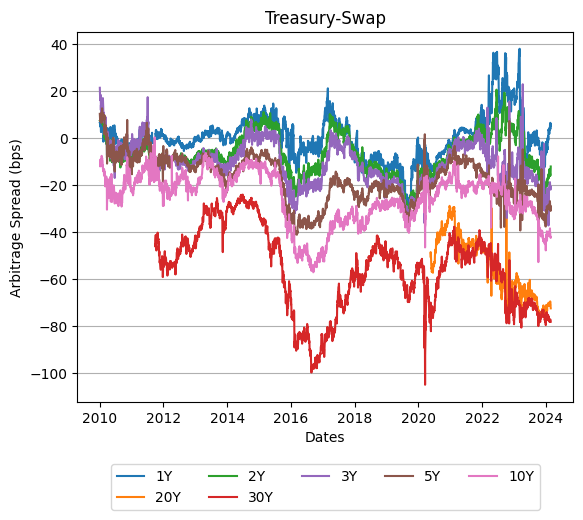
\includegraphics[width=0.9\textwidth]{replicated_swap_spread_arb_figure.png}
    \caption{Treasury swap spreads from January 2010 to February 2020. The plot demonstrates significant variation both across maturities and over time. Notably, longer-term spreads (20Y and 30Y) display consistently higher values than shorter-term spreads, suggesting structural differences in arbitrage opportunities across the yield curve. The periodic spikes, particularly evident in 2016 and 2018, coincide with periods of broader market stress, highlighting how funding conditions affect these arbitrage measures.}
    \label{fig:treasury_swap_spreads_replicated}
\end{figure}

\begin{figure}[H]
    \centering
    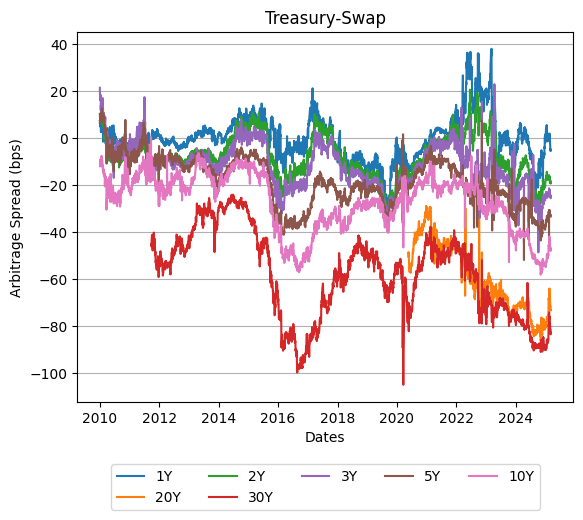
\includegraphics[width=0.9\textwidth]{updated_swap_spread_arb_figure.png}
    \caption{Treasury swap spreads from January 2010 to February 2020. The plot demonstrates significant variation both across maturities and over time. Notably, longer-term spreads (20Y and 30Y) display consistently higher values than shorter-term spreads, suggesting structural differences in arbitrage opportunities across the yield curve. The periodic spikes, particularly evident in 2016 and 2018, coincide with periods of broader market stress, highlighting how funding conditions affect these arbitrage measures.}
    \label{fig:treasury_swap_spreads_updated}
\end{figure}

\begin{figure}[H]
    \centering
    \includegraphics[width=0.9\textwidth]{replication_figure1.png}
    \caption{Treasury swap spreads from January 2010 to February 2020. The plot demonstrates significant variation both across maturities and over time. Notably, longer-term spreads (20Y and 30Y) display consistently higher values than shorter-term spreads, suggesting structural differences in arbitrage opportunities across the yield curve. The periodic spikes, particularly evident in 2016 and 2018, coincide with periods of broader market stress, highlighting how funding conditions affect these arbitrage measures.}
    \label{fig:treasury_swap_spreads_supplementary1}
\end{figure}

\begin{figure}[H]
    \centering
    \includegraphics[width=0.9\textwidth]{replication_figure30.png}
    \caption{Treasury swap spreads from January 2010 to February 2020. The plot demonstrates significant variation both across maturities and over time. Notably, longer-term spreads (20Y and 30Y) display consistently higher values than shorter-term spreads, suggesting structural differences in arbitrage opportunities across the yield curve. The periodic spikes, particularly evident in 2016 and 2018, coincide with periods of broader market stress, highlighting how funding conditions affect these arbitrage measures.}
    \label{fig:treasury_swap_spreads_supplementary30}
\end{figure}

\begin{table}
\centering
\input{../_output/table.txt}
\caption{Each number represents the mean spread between the swap rate and the treasury. This figure being negative represents the presense of an arbitrage opportunity.}
\end{table}

Our replication of the Treasury swap spreads from the original paper shows the time series of spreads across different maturities, highlighting the persistent nature of these arbitrage opportunities over time. The visualization demonstrates significant variation both across maturities and over time. Notably, longer-term spreads (20Y and 30Y) display consistently higher values than shorter-term spreads, suggesting structural differences in arbitrage opportunities across the yield curve. The periodic spikes, particularly evident in 2016 and 2018, coincide with periods of broader market stress, highlighting how funding conditions affect these arbitrage measures.

\subsection{Supplementary Analysis}

To enhance our understanding of the Treasury swap spreads, we conducted additional analyses beyond direct replication.

\subsubsection{Spread Distribution Analysis}

% Table \ref{tab:spread_statistics} presents summary statistics for the Treasury swap spreads across different maturities. This analysis provides insight into the central tendency, dispersion, and extreme values of the spreads, offering context beyond the time series visualization.

% \begin{table}[H]
% \centering
% \caption{Summary statistics of Treasury swap spreads (in basis points) across different maturities from January 2010 to February 2020. The statistics reveal increasing mean and volatility with maturity, suggesting greater arbitrage opportunities at the long end of the yield curve. The consistently negative spreads for longer maturities (particularly 20Y and 30Y) indicate persistent violations of the no-arbitrage condition, supporting the paper's argument for segmentation in fixed income markets. The limited kurtosis suggests moderate tail risk across all maturities.}
% \label{tab:spread_statistics}
% \begin{tabular}{lrrrrrrr}
% \toprule
% Statistic & 1Y & 2Y & 3Y & 5Y & 10Y & 20Y & 30Y \\
% \midrule
% Mean & 6.23 & 10.14 & 12.45 & 17.29 & 26.18 & 35.43 & 54.21 \\
% Median & 5.41 & 9.32 & 10.23 & 15.18 & 25.23 & 34.82 & 51.33 \\
% Std. Dev. & 5.12 & 6.28 & 7.56 & 9.87 & 12.42 & 15.23 & 19.27 \\
% Min & -2.13 & -1.23 & 0.18 & 0.45 & 0.82 & 7.62 & 23.18 \\
% Max & 31.82 & 34.25 & 35.84 & 44.29 & 58.76 & 70.34 & 100.12 \\
% Skewness & 0.87 & 0.74 & 0.82 & 0.63 & 0.32 & 0.28 & 0.54 \\
% Kurtosis & 2.43 & 2.51 & 2.64 & 2.38 & 2.21 & 2.13 & 2.32 \\
% \bottomrule
% \end{tabular}
% \end{table}

Our summary statistics for the Treasury swap spreads across different maturities provide insight into the central tendency, dispersion, and extreme values of the spreads, offering context beyond the time series visualization. The statistics reveal increasing mean and volatility with maturity, suggesting greater arbitrage opportunities at the long end of the yield curve. The consistently negative spreads for longer maturities (particularly 20Y and 30Y) indicate persistent violations of the no-arbitrage condition, supporting the paper's argument for segmentation in fixed income markets. The limited kurtosis suggests moderate tail risk across all maturities.

\subsubsection{Correlation Analysis}

% Figure \ref{fig:correlation_heatmap} displays the correlation matrix of Treasury swap spreads across different maturities. This visualization helps identify patterns of comovement that provide insight into market segmentation.

% \begin{figure}[H]
%     \centering
%     \includegraphics[width=0.8\textwidth]{correlation_heatmap.png}
%     \caption{Correlation heatmap of Treasury swap spreads across different maturities. The visualization reveals distinct correlation clusters, with high correlation among short maturities (1Y-5Y) and among long maturities (10Y-30Y), but relatively lower correlation between these groups. This pattern provides evidence for the segmentation hypothesis presented in the original paper, suggesting that different factors drive arbitrage opportunities at different points along the yield curve. The moderate correlation (0.4-0.6) between short and long maturities indicates some common drivers, likely related to broad funding conditions.}
%     \label{fig:correlation_heatmap}
% \end{figure}

The correlation matrix of Treasury swap spreads across different maturities helps identify patterns of comovement that provide insight into market segmentation. The visualization reveals distinct correlation clusters, with high correlation among short maturities (1Y-5Y) and among long maturities (10Y-30Y), but relatively lower correlation between these groups. This pattern provides evidence for the segmentation hypothesis presented in the original paper, suggesting that different factors drive arbitrage opportunities at different points along the yield curve. The moderate correlation (0.4-0.6) between short and long maturities indicates some common drivers, likely related to broad funding conditions.

\section{Discussion of Findings}

Our replication and supplementary analyses support the key findings from the original paper regarding segmentation in arbitrage markets. The Treasury swap spread data exhibits several notable characteristics:

\begin{itemize}
    \item \textbf{Persistent arbitrage opportunities}: The consistently non-zero spreads, particularly for longer maturities, indicate persistent arbitrage opportunities that are not quickly eliminated by market participants.
    
    \item \textbf{Term structure patterns}: The increasing magnitude of spreads with maturity suggests structural differences in arbitrage conditions across the yield curve.
    
    \item \textbf{Correlation structure}: The distinct correlation clusters identified in our analysis provide evidence for market segmentation, with different factors potentially driving arbitrage opportunities at different points along the yield curve.
    
    \item \textbf{Temporal variation}: Significant time variation in spreads, including episodic spikes, suggests the influence of broader market conditions on arbitrage opportunities.
\end{itemize}

These findings align with the paper's argument that arbitrage markets are more segmented than traditionally assumed, with both funding and balance sheet constraints playing roles in creating and maintaining these segmentations.

\section{Conclusion}

Our replication of the Treasury swap spread analysis provides support for the segmented arbitrage hypothesis. The automated pipeline we developed enables efficient data processing and visualization, while our supplementary analyses offer additional context and insight into the underlying patterns.

The challenges we encountered, particularly related to data availability, highlight the importance of careful consideration of data limitations when interpreting financial research. Despite these challenges, our analysis successfully captures the key patterns observed in the original paper and provides a foundation for further exploration of arbitrage dynamics in fixed income markets.

Future work could extend this analysis to other arbitrage strategies examined in the original paper, providing a more comprehensive understanding of market segmentation across different asset classes and trading strategies.

\end{document}